\chapter{LƯA CHỌN PHƯƠNG ÁN}
    \section{Lựa chọn phương án cơ khí}
        \subsection{Yêu cầu phương án cơ khí}
            \begin{itemize}
                \item Đảm bảo độ bám đường, khó lật khi vào cua với tốc độ cao.
                \item Thuật toán điều khiển đơn giản.
                \item Kết cấu cơ khí vững, nhỏ gọn, ổn định và dễ chế tạo.
                \item Chủ động trong việc chuyển hướng, chuyển hướng tốt. 
            \end{itemize}
        \subsection{So sánh các sơ đồ nguyên lý}
            \hspace*{0.6cm}Xét theo từng sơ đồ nguyên lý đã tìm hiểu trong phần tổng quan, bảng dưới đây 
                            trình bày ưu và nhược điểm của từng loại sơ đồ:
            \begin{longtable}{|p{4cm}|p{5cm}|p{5cm}|}
                \caption{So sánh các sơ đồ nguyên lý robot} 
                \label{tab:compare_robot_schemes} \\ 
                \hline
                \textbf{Sơ đồ nguyên lý} & \textbf{Ưu điểm} & \textbf{Nhược điểm} \\
                \hline
                \endfirsthead
                \hline
                \textbf{Sơ đồ nguyên lý} & \textbf{Ưu điểm} & \textbf{Nhược điểm} \\
                \hline
                \endhead
                \hline
                \endfoot
                \hline
                \endlastfoot
                Robot Zumo Slim \newline
                \textit{Phương án 1} \newline
                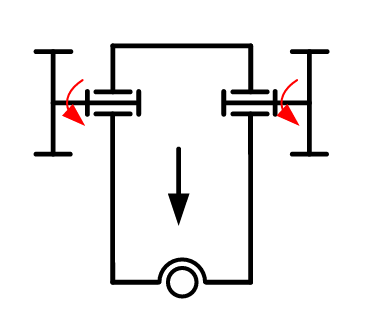
\includegraphics[width=3cm]{pictures/chapter2/chapter2_pic_1.png} & 
                - Kết cấu 3 bánh nhỏ gọn, đơn giản \newline
                - Mô hình toán đơn giản, dễ điều khiển \newline
                - Đảm bảo xe luôn được đồng phẳng & 
                - Khả năng bám đường không tốt, vào cua ở tốc độ cao dễ bị trượt. \newline
                - 2 bánh sau vừa dẫn động vừa dẫn hướng, trọng tâm không nằm trên trục bánh sau dẫn tới dễ bốc đầu khi chạy ở tốc độ cao. \\
                \hline
                Robot Pinto \newline
                \textit{Phương án 2} \newline
                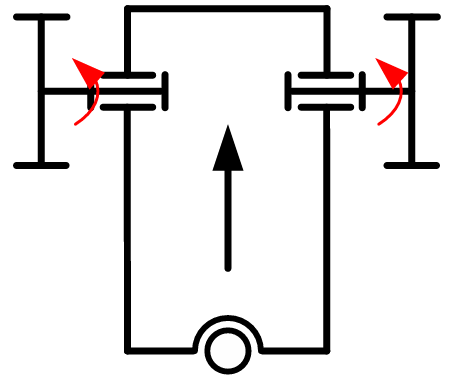
\includegraphics[width=3cm]{pictures/chapter2/chapter2_pic_2.png} & 
                - Kết cấu 3 bánh nhỏ gọn, đơn giản \newline
                - Mô hình toán đơn giản, dễ điều khiển \newline
                - Đảm bảo xe luôn được đồng phẳng & 
                - Khả năng bám đường không tốt, vào cua ở tốc độ cao dễ bị trượt. \newline
                - Do dẫn động nằm phía trước nên giảm thời gian phản ứng khi dò line. \\
                \hline
                Robot Newbie \newline
                \textit{Phương án 3} \newline
                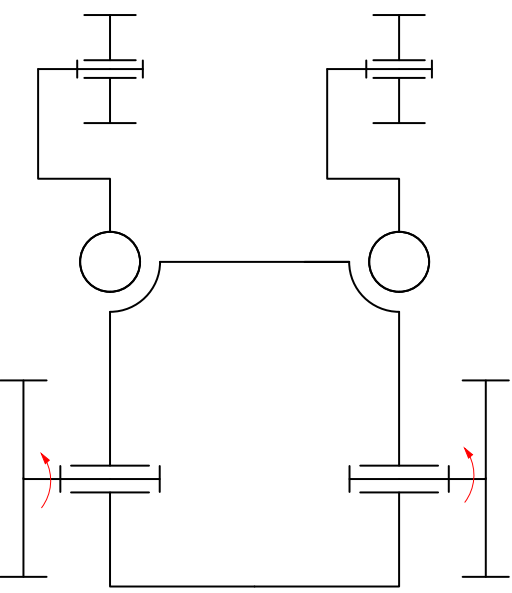
\includegraphics[width=2.5cm]{pictures/chapter2/chapter2_pic_3.png} & 
                - Kết cấu 4 bánh giúp tăng khả năng tải. \newline
                - Khả năng vào cua và bám đường tốt. \newline
                - Kết cấu cơ khí đơn giản & 
                - Đảm bảo đồng trục 2 bánh dẫn động. \newline
                - Đảm bảo đồng phẳng giữa các bánh xe. \newline
                - Bị hóc đầu nếu đặt tải lệch về phía sau. \newline
                - Dễ bị lật khi vào cua với tốc độ cao. \newline
                - Mô hình tính toán phức tạp, khó điều khiển. \\
                \hline
                Robot FireBall \newline
                \textit{Phương án 5} \newline
                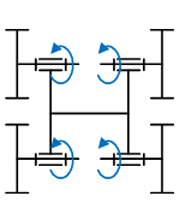
\includegraphics[width=2.5cm]{pictures/chapter2/chapter2_pic_4.png} &
                - Kết cấu cơ khí đơn giản, cân bằng tốt. \newline
                - Tải chia đều cho 4 động cơ -> giảm tải. \newline
                - Điều khiển tùy ý dễ dàng. &
                - Đảm bảo đồng trục cả 2 bánh trước và 2 bánh sau. \newline
                - Đảm bảo đồng phẳng giữa các bánh. \newline
                - Mô hình tính toán phức tạp, khó điều khiển. \\ 
                \hline
                Robot Khepera IV \newline
                \textit{Phương án 4} \newline
                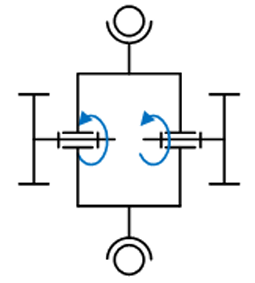
\includegraphics[width=2.5cm]{pictures/chapter2/chapter2_pic_5.png} &
                - Kết cấu 4 bánh đơn giản, mô hình toán đơn giản, dễ điều khiển.\newline 
                - Trọng tâm nằm ngay trục dẫn động giữ kết cấu dễ ổn định. &
                - Khả năng vào cua kém. \newline
                - Đảm bảo đồng trục giữa 2 bánh dẫn động và đồng phẳng giữa các bánh. \newline
                - Hai bánh giữa chịu áp lực lớn vừa chịu tải vừa kéo tải. \\
                \hline
                
            \end{longtable}
        \subsection{Số bánh}
            \begin{longtable}{|p{4cm}|p{5cm}|p{5cm}|}
                \caption{So sánh số lượng bánh xe robot} 
                \label{tab:compare_robot_wheels} \\ 
                \hline
                \textbf{Số bánh} & \textbf{Ba bánh} & \textbf{Bốn bánh} \\
                \hline
                \endfirsthead
                \hline
                \textbf{Số bánh} & \textbf{Ba bánh} & \textbf{Bốn bánh} \\
                \hline
                \endhead
                \hline
                \endfoot
                \hline
                \endlastfoot
                \textbf{Ưu điểm} &
                - Yêu cầu về đồng phằng đáp ứng dễ dàng. \newline
                - Mô hình xe có kết cấu đơn giản. &
                - Khả năng bám đường tốt, khả năng ít bị lật khi vào cua. \newline
                - Khi sử dụng vi sai thì vấn đề đồng trục hai bánh sau có thể được bỏ qua. \\
                \textbf{Nhược điểm} &
                - Khả năng bám đường không tốt, khi vào cua dễ bị lật. \newline
                - Phải đảm bảo hai bánh sau đồng trục để thỏa yêu cầu xe chạy không đảo, lắc. &
                - Mô hình xe có kết cấu phức tạp (nhất là khi sử dụng vi sai). \newline 
                - Phải đảm bảo đồng phẳng cho cả bốn bánh. \\ 
            \end{longtable}
        \subsection{Vật liệu}
            \begin{table}[H]
                \centering
                \begin{tabular}{|c|p{3cm}|p{3cm}|p{3cm}|p{3cm}|}
                    \hline
                    \textbf{Vật liệu} & Gỗ & Mica & Nhôm & Inox \\
                    \hline
                    \textbf{Ưu điểm} 
                    & Nhẹ nhất trong 3 loại vật liệu được liệt kê, dễ dàng gia công, không dẫn điện, an toàn, không gây chập mạch.  
                    & Chịu được ẩm, chịu được nhiệt độ cao, chịu được lực, không dẫn điện không gây chập mạch, dễ gia công.
                    & Độ bền cao, chắc chắn, nhẹ hơn so với các kim loại khác, có thể sơn phủ để tăng tính thẩm mĩ.
                    & Độ bền cao, chắc chắn. \\
                    \hline
                    \textbf{Nhược điểm} 
                    & Dễ bị tác động bởi môi trường, khả năng chống va đập thấp.
                    & Dễ trầy xước.
                    & Giá thành gia công cao.
                    & Giá thành gia công cao. \\
                    \hline
                \end{tabular}
                \caption{So sánh các loại vật liệu chế tạo robot}
                \label{tab:label}
            \end{table}
        \hspace*{0.6cm}\textbf{Kết luận}: sau khi phân tích các phương án kết cấu cơ khí cùng với yêu cầu được đặt ra về vận tốc không cao, không phải chịu tải nặng. Nhóm quyết định xe 3 bánh, 2 bánh dẫn động ở phía trước và 1 bánh dẫn hướng phía sau để đảm bảo đồng phẳng và dễ điều khiển theo cơ cấu Pinto. Vật liệu được nhóm lựa chọn để thiết kế khung xe với yêu cầu kỹ thuật trên là nhôm với độ dày 2mm. 
    \section{Lựa chọn phương án điện}
        \subsection{Lựa chọn cảm biến dò line}
            \subsubsection{Yêu cầu cảm biến}
                \begin{itemize}
                    \item Đáp ứng nhanh khi nhận biết sự thay đổi màu sắc giữa trắng và đen trên sa bà.
                    \item Tín hiệu cảm biến trả về nhanh để giúp xe kịp thời chuyển hướng ở những đoạn line uốn cong.
                    \item Tín hiệu đọc về dạng analog, ít nhiễu. Giải thuật đơn giản.
                    \item Dễ tìm thấy trên thị trường, giá thành hợp lý. 
                \end{itemize}
            \subsubsection{Kết luận}
                \hspace*{0.6cm}Sau khi phân tích về ưu nhược điểm của ba phương án cảm biến dò line ở chương 
                                1, nhóm quyết định lựa chọn cảm biến IR TCRT5000, đồng thời thiết kế mạch PCB có 
                                tính toán số lượng cảm biến, khoảng cách giữa các cảm biến và độ cao gá đặt cảm biến tới mặt line
            \subsubsection{Cảm biến hồng ngoại TCRT5000}
                \begin{figure}[H]
                    \centering
                    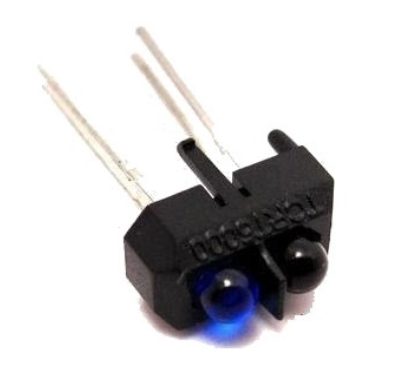
\includegraphics[width=0.25\textwidth]{pictures/chapter2/chapter2_pic_6.png}
                    \caption{Cảm biến hồng ngoại TCRT5000}
                    \label{fig:tcrt5000}
                \end{figure}
                \hspace*{0.6cm}Cảm biến hồng ngoại TCRT5000 là cảm biến quang điện có khả năng phát hiện vật thể dựa trên sự phản xạ của ánh sáng hồng ngoại. Cảm biến này bao gồm một LED hồng ngoại và một phototransistor, cho phép nó phát hiện sự hiện diện của vật thể trong khoảng cách từ 0 đến 25 cm. 
        \subsection{Phương án bố trí cảm biến dò line}
            \subsubsection{Các phương án bố trí cảm biến}
                \begin{itemize}
                    \item Bố trí dạng ma trận:
                    \begin{figure}[H]
                        \centering
                        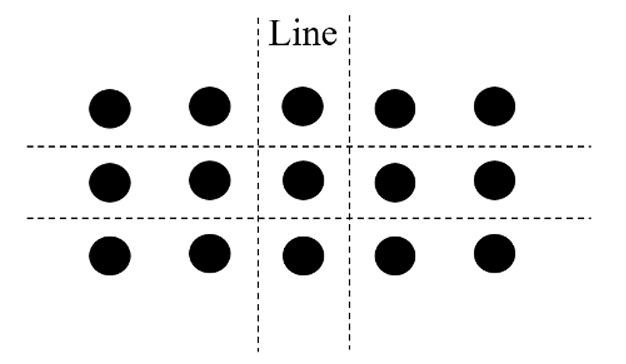
\includegraphics[width=0.5\textwidth]{pictures/chapter2/chapter2_pic_7.png}
                        \caption{Bố trí cảm biến dạng ma trận}
                        \label{fig:matrix_sensor_layout}
                    \end{figure}
                    \item Bố trị dạng đường thẳng:
                    \begin{figure}[H]
                        \centering
                        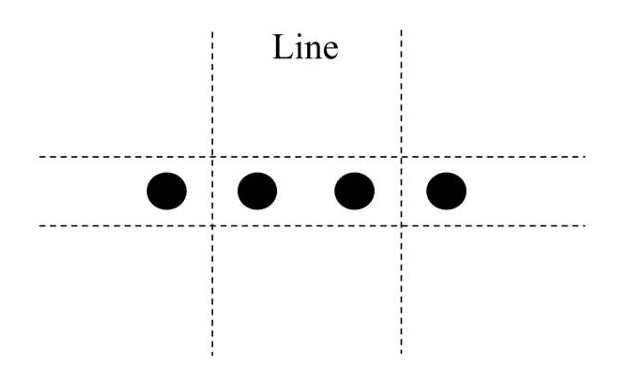
\includegraphics[width=0.5\textwidth]{pictures/chapter2/chapter2_pic_8.png}
                        \caption{Bố trí cảm biến dạng đường thẳng}
                        \label{fig:line_sensor_layout}
                    \end{figure}
                    \item Bố trí dạng chữ V:
                    \begin{figure}[H]
                        \centering
                        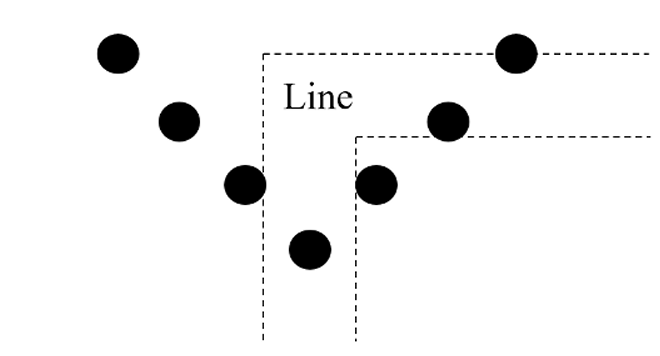
\includegraphics[width=0.5\textwidth]{pictures/chapter2/chapter2_pic_9.png}
                        \caption{Bố trí cảm biến dạng chữ V}
                        \label{fig:v_sensor_layout}
                    \end{figure}
                \end{itemize}
                \begin{table}[H]
                    \centering
                    \begin{tabular}{|p{3cm}|p{5cm}|p{5cm}|}
                        \hline
                        \textbf{Dạng bố trí} & \textbf{Ưu điểm} & \textbf{Nhược điểm} \\
                        \hline
                        \textbf{Dạng ma trận} &
                        - Thu được nhiều thông tin để nội suy hay so sánh làm tăng độ chính xác \newline
                        - Có thể dự đoán trước được đường đi &
                        - Sử dụng nhiều cảm biến. \newline
                        - Khối lượng xử lý lớn, thuật toán xử lý phức tạp. \\ 
                        \hline
                        \textbf{Dạng đường thẳng} &
                        - Thuật toán đơn giản.  \newline
                        - Phát hiện được các đoạn giao. \newline
                        - Được sử dụng phổ biến.  &
                        - Xử lý những đoạn cua gắt kém. \\
                        \hline
                        \textbf{Dạng chữ V} &
                        - Thích hợp cho đường line có nhiều đoạn cua gắt (lớn hơn 90 độ). &
                        - Ít được sử dụng phổ biến. \newline
                        - Giải thuật xử lý phức tạp hơn so với dạng đường thẳng. \\ 
                        \hline
                    \end{tabular}
                    \caption{Mô tả bảng}
                    \label{tab:label}
                \end{table}
            \subsubsection{Kết luận}
                \hspace*{0.6cm}Với sa bàn được yêu cầu trên đầu bài, bề rộng line là 26 mm với các khúc cua đơn giản, không phức tạp, nhóm lựa chọn bố trí cảm biến theo dạng đường thẳng. 
        \subsection{Lựa chọn giải thuật xác định tọa độ line}
            